\documentclass{llncs}
\usepackage[utf8]{inputenc}
\usepackage{todonotes}
\usepackage{makeidx}  % allows for indexgeneration
\usepackage{dirtytalk}
\usepackage{color}
\usepackage{glossaries}
\usepackage{graphicx}
\usepackage{float}
\usepackage{booktabs}
\usepackage[caption = false]{subfig}
\graphicspath{ {images/} }
\usepackage{rotating}
\usepackage{pdflscape}


% Reset footnotes every page
%\usepackage{perpage}
%\MakePerPage{footnote}

\begin{document}
\frontmatter

%%%%%%%%%%%%%%%%%%%%%%%%
%%%%%%%  HEADER  %%%%%%%
%%%%%%%%%%%%%%%%%%%%%%%%
\title{Malware Detection Via Machine Learning}
\subtitle{}
\titlerunning{Malware Detection Via ML}
\author{João F. Godinho}
\institute{Instituto Superior Técnico\\
\email{joao.f.godinho@tecnico.ulisboa.pt}}
\let\oldaddcontentsline\addcontentsline
\def\addcontentsline#1#2#3{}
\maketitle
\def\addcontentsline#1#2#3{\oldaddcontentsline{#1}{#2}{#3}}
%\todo[inline]{Validate the title, subtitle}

%%%%%%%%%%%%%%%%%%%%%%%%
%%%%%%% ACRONYMS %%%%%%%
%%%%%%%%%%%%%%%%%%%%%%%%
\newacronym{hids}{HIDS}{Host-based Intrusion Detection Systems}
\newacronym{ml}{ML}{machine learning}
\newacronym{caro}{CARO}{Computer Antivirus Research Organization}
\newacronym{ai}{AI}{Artificial Intelligence}
\newacronym{api}{API}{Application Programming Interface}
\newacronym{bios}{BIOS}{Basic Input/Output System}
\newacronym{dll}{DLL}{Dynamic-Link Library}
\newacronym{cc}{CC}{Creative Common's}
\newacronym{ann}{ANN}{Artificial Neural Networks}
\newacronym{tpr}{TPR}{True Positive Rate}
\newacronym{fpr}{FPR}{False Positive Rate}
\newacronym{svm}{SVM}{Support Vector Machine}
\newacronym{mist}{MIST}{Malware Instruction Set}
\newacronym{lr}{LR}{Logistic Regression}
\newacronym{pe}{PE}{Portable Executable}

%%%%%%%%%%%%%%%%%%%%%%%%
%%%%%%% ABSTRACT %%%%%%%
%%%%%%%%%%%%%%%%%%%%%%%%
\begin{abstract}
	Malware, which focuses on harming or subverting a system, has grown exponentially in recent years. The regular signature and heuristic methods applied by anti-virus vendors can fall short on keeping up with the rise of new types of malware. Other works have shown that machine learning has potential for dealing with the task of malware detection. With this in mind, the current report elaborates on the problem of malware, how anti-virus detect it, and proposes the development of a machine learning system to deal with the task of malware detection. To design the system to be, the current work will make use of a dataset with 388,513 samples for training and evaluation, focusing on how laboratory and real-world conditions can affect the final result.
\end{abstract}


\setcounter{tocdepth}{2}
\tableofcontents



\mainmatter
%%%%%%%%%%%%%%%%%%%%%%%%
%%%%%%%  INTRO   %%%%%%%
%%%%%%%%%%%%%%%%%%%%%%%%

% Temporary quotes, move to bib
% 1 - Attacking Malicious Code: A report to the Infosec Research Council
% 2 - AV-TEST Security Report 2015/2016 - https://www.av-test.org/fileadmin/pdf/security_report/AV-TEST_Security_Report_2015-2016.pdf
% 3 - McAfee Labs Threats Report April 2017 - https://www.mcafee.com/us/resources/reports/rp-quarterly-threats-mar-2017.pdf
% 4 - Symantec Internet Security Threat Report - https://www.symantec.com/content/dam/symantec/docs/reports/istr-22-2017-en.pdf
% 5 - Scanners of The Year 2000: Heuristics - http://vxheaven.org/lib/adg00.html
% 6 - Thomas Mitchell - Machine Learning
% 7 - Some Studies in Machine Learning Using the Game of Checkers - Arthur L. Samuel - http://citeseerx.ist.psu.edu/viewdoc/download?doi=10.1.1.368.2254&rep=rep1&type=pdf
% 8 - Prudent Practices for Designing Malware Experiments: Status Quo and Outlook

\section{Introduction}\label{sec:introduction}
Malware, which can be referred to by other names like malicious software or malicious code, can be described as \say{any code added, changed, or removed from a software system in order to
intentionally cause harm or subvert the intended function of the system}\cite{mcgraw:mal_code}. Malware can be a piece of code attached to a legitimate program, an independent program, or a combination of both. The reasoning that leads to malware creation varies greatly, some are created to demonstrate some vulnerability or concept and do not cause direct harm to systems, while others are used to steal information or render systems useless. The wide variety and quantity of now-a-day systems and the amount of sensitive information they store provide numerous opportunities to illegally make a profit out of subverting legitimate systems.

The amount of malware has shown an exponential increase since the early 2000s, from 1.7 million in 2005 to over 600 million by the end of 2016\cite{av-test:report,mcafee:report}. According to a 2007 study by McAfee\footnote{McAfee Study Finds 4 Percent of Search Results Malicious, by Frederick Lane, June 4, 2007 [http:\/\/www.newsfactor.com\/story.xhtml?story\_id=010000CEUEQO]} about 4\% of the query results by major search engines lead to potentially dangerous websites. A more recent study by Norton in 2010\footnote{Symantec Press Release, July 29, 2010 [https://www.symantec.com/en/aa/about/newsroom/press-releases/2010/symantec\_0729\_02]} showed that at least 10\% of top trending search terms returned malicious results. From the contact with malicious software, 1.1 billion identities (i.e. user's personal information) have been exposed in 2016 alone\cite{symantec:report}.


Given the wide range and quantity of systems being operated by naive users, in the sense that they lack the knowledge to distinguish malicious and legitimate software, the first line of defense against threats are \gls{hids}, commonly known as anti-virus solutions. Their main function is to prevent infections by malicious code, which is achieved by detecting a program as malicious and disallow it from running (i.e. quarantining the malicious file).

To detect malicious software, anti-virus solutions depend on two main methods. \textit{Signature-based} methods check for the presence of unique byte sequences from known malware. For this method to be effective, a database of all malware signatures must be available, which leads to an obvious shortcoming: only known malware is detected\cite{gryaznov:scanners}. New and unknown malware is not detected until vendors analyze it and update their clients. To improve the effectiveness of anti-virus and overcome the problem in aforementioned methods, \textit{heuristic-based} methods are employed. These apply a set of rules to decide whether a program is likely to be malware or not. Like before, a database of rules must be available, but unlike signature methods, which provide exact matching on malware, heuristic methods are capable, to some degree, of generalizing malware features, hence detecting new and unknown malware. Although more sophisticated, heuristic-based methods need a database of rules that must be defined \textit{a priori}, just like signature methods.

As mentioned before, signature methods only detect known malware, which translates to a very low false positive rate (i.e. goodware wrongly classified as malware), while having a high detection rate (i.e. correctly classified malware from the total malware), assuming the signature database is on par with malware samples, which at the rate new malware emerges becomes a hard task. For heuristic methods new and unknown malware can be detected due to similarities to known malware, translating to a higher detection rate with less information, but with the downside of raising the false positive rate, as benign programs (goodware) can be flagged malicious due to characteristics that fit into malware rules\cite{gryaznov:scanners}. To improve the effectiveness of anti-virus, both methods must complement each other.

Having the need to either create signatures for new malware or define a set of rules that describe malware characteristics becomes a cumbersome task for the increasing malware numbers. To try and improve the detection task of anti-virus software, the current work proposes a \gls{ml} approach to malware detection as an evolution to heuristic-based methods.

The machine learning field studies the development of computer programs that automatically improve with experience. A program is given a task and an experience, if its performance at the task improves with the experience given, then the program is learning the task\cite{mitchell:ml}. In the proposed work, the task at hand is to distinguish malware from goodware (i.e. classify samples) and the experience is a wide variety of samples, both goodware and malware. The final result is a program that performs well for the given task (i.e. successfully learns to distinguish goodware from malware).

The \gls{ml} field has been around for multiple decades, with some of the earlier works dating back to 1959 by Arthur L. Samuel\cite{samuel:studies}, but only in recent years has the field grown in popularity. Its recent growth can be accredited to two main factors: availability of large data sets and computation power. Larger data sets provide more experience for a program to learn from, but also require more processing power.

The growing number of malware samples provide a good opportunity to make use of \gls{ml} for malware detection. This approach is not new and has provided high detection rates with low false positive rates\cite{miller:rev_int,nissim:al_pdf,perdisci:behavior,rieck:dynamic,schultz:data_mining}. However, many of the resulting research is done under laboratory conditions that do not represent real world scenarios. Some of those conditions have been studied in \cite{rossow:practices} and include the correctness of datasets, transparency and realism. Alongside the application of \gls{ml} to detect malware, the proposed work will study how laboratory conditions differ from real world one's and how effectiveness is affected.

To provide a solution that makes use of \gls{ml} to detect malware and its performance under laboratory \textit{vs.} real world conditions, the proposed work will follow an approach that is divided into three stages:

\begin{itemize}
	\item \textit{Data collection}: experience from which a program can learn must be available, as such the first step must ensure the collection of samples that represent both malware and goodware examples. The current work will take advantage of the Malwr\cite{tool:malwr} service, which provides both static (e.g. library imports) and dynamic (e.g. library call order during runtime) details about a sample. The total number of available samples surpasses 388 thousand, dated from April 2013 to October 2016.
	\item \textit{Data labeling}: before training a classifier to detect malware, samples must be labeled as either benign or malign. The Malwr\cite{tool:malwr} service provides details on how multiple anti-virus solutions classify a sample, hence the approach is to use said classification to determine the legitimacy of a sample. This step is not linear, as different anti-virus classify samples differently, introducing edge cases (e.g. 50\% classify malware, the other 50\% classify goodware). To overcome this, the current work must develop a metric to deal with such cases.
	\item \textit{Classifier implementation}: at this stage the collected data is ready to be used as experience for the program. Using static and dynamic details together with the labeling of the samples, a classifier can be trained to distinguish between malware and goodware. Alongside the classifier creation, this phase must also measure the effectiveness of the solution. For this work's scope, the effectiveness is to be measured under laboratory and real world conditions.
\end{itemize}

In sum, the work to be done as to verify the application of \gls{ml} methods for the task of detecting malware is: collection of samples, labeling of collected samples and finally usage of the resulting dataset to achieve a malware classifier.

The following sections provide deeper analysis on the subject of using \gls{ml} to classify malware, as well as the choices to be made and the reasoning behind them. Section \ref{sec:related_work} describes related work that both influenced and motivated the current work. Section \ref{sec:solution} details the intended approach, the tools to be used, how the work is to be presented and the already accomplished work. Section \ref{sec:conclusion} summarizes and closes the report.

%\todo[inline]{falar dos antivirus para combater isto, falar nas tecnicas basicas: signature based, heuristic based. tirar partido de ML para estender metodos heuristicos e melhorar a classificaçao de malware.}
%
%
%\todo[inline]{one liner do que é malware (quote), quantificar (quote), necessidade de detectar malware mais rapidamente (automatizar/generalizar).
%
%Avanços na detecçao do malware, pouca coisa. Aplicaçao de ML neste tipo de problema.
%
%Contributos do trabalho para este problema, desenvolver um classificador que funcione no mundo real e ajude a resolver o problema.
%
%1. Dados recolhidos, o que posso extrair dos dados\\
%2. Definir o que é malware (thresholds, consenso)\\
%3. Comparaçao de metodologias (estatatica/dinamica)}

%%%%%%%%%%%%%%%%%%%%%%%%
%%%%%%% RELATED  %%%%%%%
%%%%%%%%%%%%%%%%%%%%%%%%
\section{Related Work}\label{sec:related_work}

% #1 Semantics-Aware Malware Detection
% #2 Attacking Malicious Code: A report to the Infosec Research Council
% #3 Malware, Rootkits & Botnets A Beginner's Guide pp.10
% #4 Computer viruses: theory and experiments
% #5 Theory of self-reproducing automata
% #6 The Evolution of Viruses and Worms
% #7 The art of computer virus research and defense
% #8 https://www.av-test.org/en/
% #9 http://www.caro.org/articles/naming.html
% #10 http://members.chello.at/erikajo/vnc99b2.txt
% #11 Learning to Detect and Classify Malicious Executables in the Wild
% #12 The Evolution of Viruses and Worms
% #13 http://cert.europa.eu/static/SecurityAdvisories/2017/CERT-EU-SA2017-012.pdf
% #14 https://www.virusbulletin.com/uploads/pdf/magazine/2002/200201.pdf

%%%%%%%%%%%%%%%%%%%%%%%%%%%%%%%%%%%%%%%%%%%%%%%%%%%%%%%%%%%%%%%%%%%%%%%%%%
%%% Background
\subsection{Background}\label{subsec:background}
Malware, which can be referred to by other names like malicious software or malicious code, can be described as \say{a program that has malicious intent}\cite{christodorescu:semantics}, or more detailed as any code added, changed, or removed from a software system in order to intentionally cause harm or subvert the intended function of the system\cite{mcgraw:mal_code}.

The term malware was first used by Yisrael Radai in 1990\cite{elisan:malware}, before then malicious software was referred to as computer viruses, a notion which was first formalized by Cohen in 1983\cite{cohen:virus}. Given term computer virus predates the term malware, it is not uncommon to see both terms used interchangeably. For the purpose of this work the term malware is adopted, for reasons explained in the following paragraphs.

To the exponential growth of malware\cite{av-test:report}, the ability to distinguish between malware samples is crucial. In the biological world, different types of infections reckon distinctive disinfections, the same applies to the digital world. The infection method, behavior and subsequently purpose of malware samples vary, hence being able to make a distinction facilitates prevention and disinfection by anti-virus solutions.

There exists no ground truth when it comes to distinguishing malware, leading to subtle differences on the classification and naming of the same malware instance by different parties. To facilitate the reader's understanding of the topic, the current work will focus on defining malware types based on their propagation and purpose.

With respect to the propagation method, malware can be split into three classes\cite{kolter:learning}.

\paragraph{Virus.}\footnote{This work uses virus as a subset of malicious code, hence the choice of using the term malware over virus.}This type of malware inherits its name from resembling to biological viruses. A virus is usually composed by two main subroutines. The first subroutine is responsible for infecting other programs by attaching the virus code, while the second subroutine is the actual malware payload that contains the malware purpose (i.e. virus payload)\cite{chen:evolution}. Viruses are attached to programs and propagate when an infected program is run, hence depending on other programs (as hosts) and user interaction. For viruses to infect new systems, an infected file must be carried between them by a user (e.g. USB pen, email attachment), reinforcing the user's role in this propagation method.

\paragraph{Worm.} The increasing number of network connected devices facilitates the application of worms to propagate malware. A worm shares the self-replicating ability of viruses, but discards user interaction and the need for a host. This is possible by making a worm an independent program that exploits networks to find vulnerable systems to infect with a copy of themselves\cite{chen:evolution}. Similarly to viruses, worms can contain additional payload to perform malicious actions on infected systems (e.g. Blaster worm exploited a vulnerability in RPC for propagation while its payload flooded a Microsoft domain\footnote{W32/Blaster worm, CERT, August 11, 2003 [http://www.cert.org/historical/advisories/CA-2003-20.cfm]}).

\paragraph{Trojan.} While viruses and worms focus on self-propagation, trojans focus on deceiving users into executing them, disregarding propagation. Trojans try to appeal users with some useful functionality as to allure into running the program\cite{szor:art}. By hoaxing users into running them, trojans bypass the need for a host (in the virus case) or an exploit (in the worm case) to perform malicious actions.\\

These three classes are not exclusive and can be used in conjunction to facilitate propagation (e.g. a virus that relies on a trojan to start propagating). Given the inexistent standards for malware naming, some literature\cite{szor:art} define worms as a subset of viruses, as some worms start by attaching to files. With the general infection methods layered out, the following will succinctly describe the general naming when referring to the malware purpose (i.e. its payload).

Given the high numbers of malware multiple purposes imply multiple names, as such the following lists some of the most commonly heard names and definitions as given by McAfee\cite{mcafee:glossary}:

\begin{itemize}
	\item \textit{Adware}: Program that automatically displays advertisement to the user. Most do not cause direct harm.
	\item \textit{Backdoor}: Installs or takes advantage of an unknown entry point to a user's system, allowing remote control of a system.
	\item \textit{Dropper}: Program that facilitates the introduction of other malware instances into a system.
	\item \textit{Keylogger}: Program that monitors a user's input (e.g. keyboard strokes) to steal private information.
	\item \textit{Password Stealer (PWS)}: Program that specifically targets a user's personal information, like usernames and passwords.
	\item \textit{Ransomware}: Program that restricts access to a system/files (usually by encryption) and demands a ransom to allow a user his access.
	\item \textit{Rootkit}: Program designed to hide the existence of other (malicious) programs, hindering detection of malicious applications.
	\item \textit{Scareware}: Program that fakes the existence of malware and tricks the user into paying for disinfection or into downloading real malware.
	\item \textit{Spyware}: Program that spies on a user's activity through multiple vectors (e.g. taking prints of a user's desktop/webcam).
\end{itemize}

The ability to name a malware given its propagation method and purpose facilitates detection and disinfection, but given the high quantities of malware, being able to particularly discriminate an instance is helpful. To that purpose, attempts have been made to create naming conventions for malware.

One of the first attempts was made in 1991, by the \gls{caro}\cite{caro:naming}. This attempt was aimed at viruses only and focused on discriminating and relating virus samples. The convention defines an hierarchical naming with three levels. The base of the hierarchy is the family name, where structurally similar virus should be grouped. To further distinguish instances, a group name and major variant name is applied. To differentiate versions of the same instance and provide additional information about a sample, minor variant name and modifier fields are to be used. In sum, a virus name should look as following:

\begin{center}\texttt{family.group.major.minor:modifier}\end{center}

To enable differentiation from other types of malware, an improvement to \gls{caro}'s naming was proposed in 1999 by Geral Scheidl\cite{scheidl:naming}. Scheidl's proposal included a prefix that consisted of the platform targeted by the malware and a type (i.e. previously defined classes and names), rendering a more in-depth name:

\begin{center}\texttt{platform.type/family.group.major.minor:modifier}\end{center}

In the Virus Bulletin magazine of January 2002\cite{virus_bulletin} the naming problem is again addressed, referencing that only a small number of vendors apply \gls{caro}'s names and that the lack of cooperation between anti-virus vendors lead to multiple aliases for malware names. Again a naming convention is proposed with focus on detail by using three levels of information: malware name, classification and full text description.

Given that no naming convention is widely adopted, anti-virus vendors make use of their own naming that although similar, vary slightly. This variation raises the redundancy for instances of the same malware as shown by an article published by Symantec in 2002\footnote{A Virus by Any Other Name: Virus Naming Pratices, Costin Riau, June 2, 2002 [https://www.symantec.com/connect/articles/virus-any-other-name-virus-naming-practices]}, stating that the same malware instance has an average of four different names.

The naming problem, although not directly related to the current work, must be taken into consideration as to not influence the classification results.

%%%%%%%%%%%%%%%%%%%%%%%%%%%%%%%%%%%%%%%%%%%%%%%%%%%%%%%%%%%%%%%%%%%%%%%%%%
%%% Malware detection
\subsection{Malware Detection}\label{subsec:mal_detec}

In section \ref{sec:introduction} a brief description of malware detection methods was given. This section will provide a deeper description of detection methods, from the simplest techniques to more complex ones. The following is based on the work by Peter Szor, \textit{The Art of Computer Virus Research and Defense}\cite{szor:art}.

To detect malware instances, anti-virus applications are used. These can also be called scanners, as early detection methods simply scanned for byte sequences to detect malware. Before going into details on the different detection techniques, it is worth mentioning that scanners can be used as \textit{on-demand} or \textit{on-access} scanners. On-demand anti-virus are executed only at the user's request. On-access anti-virus are memory-resident, meaning they load as an application and intercept actions related to file and disk access. This makes it so that when files are opened, created or closed, the anti-virus scans the changed object.

\subsubsection{First-Generation Scanners.} These type of scanners work at a fairly simple level and focus searching for known byte sequences (i.e. known to be malware sequences). The applied principles include:

\paragraph{String Scanning.} A sequence of bytes that is common in a malicious program but not in a regular program is matched against a suspicious file. 

\paragraph{Wildcards.} This method is similar to string scanning, but instead of searching for a fixed sequence of bytes, a more flexible matching is made, allowing to skip bytes or byte ranges. The method can also include the use of regular expressions for matching.

\paragraph{Mismatches.} Also similar to string scanning, yet there can be $N$ number of bytes in the string that can take any value and in any position (e.g. the string \say{\texttt{01 02}} with mistmatch of 1 matches \say{\texttt{01 AA}} and \say{\texttt{AA 02}}).

\paragraph{Generic Detection.} This method typically applies both wildcards and mismatches to create generic strings that can scan for several variants of a family of malware.

\paragraph{Hashing.} This term is not a method by itself, but techniques that speed up searching algorithms, enhancing previous methods.

\paragraph{Bookmarks.} This method is both used to provide more accurate detections and disinfections. Bookmarks provide specific locations for where strings are to be searched (i.e. offsets).

\paragraph{Top-and-Tail Scanning.} Like hashing, this principle is used to speed up detection by scanning the start and end of a file, instead of the entire file. The technique is mainly effective when dealing with viruses that prefix or append data to files.

\paragraph{Entry-Point and Fixed-Point Scanning.} This technique also improves the speed of anti-virus scanners. By taking advantage of the structure of binary objects this method can start scanning at the entry-point of an object, or alternatively use the entry-point plus some fixed size as a fixed-point from where to start scanning.

\paragraph{Hyperfast Disk Access.} This last technique also provides a speed improvement. It does so by bypassing operating system level \gls{api} to read the disk directly with the \gls{bios}. It is worth noting that this technique is hard to implement nowadays due to the high variety of file systems and disk controllers.\\

The described methods, excluding the ones that focus on speed improvement, can be assigned to the signature-based type of methods, as they depend on searching some previously defined byte sequence to be effective. Their effectiveness depends on an updated knowledge base with the strings to be matched.

\subsubsection{Second-Generation Scanners.} These methods improve on the previous generation by doing an analysis at a higher level of abstraction. Where first-generation scanners would match sequences of bytes, second-generation scanners also look at the bytes representation. The applied principles include:

\paragraph{Smart Scanning.} This method takes the assembly representation of the bytes into account and instructions that have no effect (e.g. \texttt{NOP}) can be skipped. The resulting signature is smaller and more easily detects mutations. The same principle can be applied to textual malware (e.g. scripts), where extra white spaces have no effect.

\paragraph{Skeleton Detection.} This method is specifically useful in detecting textual malware (e.g. macros) families. By parsing the macro statements line by line, the scanner can drop nonessential statements. The result can be seen as a skeleton of the full macro that contains only the relevant code that appears in malware.

\paragraph{Nearly Exact Identification.} This method provides a more accurate way to detect malware. First-generation scanners base detection mainly on a byte sequence, whereas nearly exact identification makes use of double-string detection. This is specifically useful to identify same family malware. Another nearly exact identification method applies a checksum to a range from the malware body, the resulting checksum can then be used to detect and disinfection files.

\paragraph{Exact Identification.} This method enhances the previous method by adding the ability to differentiate malware variants. It does so by using as many checksum ranges as needed to identify variants of the same malware, improving the accuracy and facilitating disinfection.\\

Like in the previous generation, these methods fit into signature-based, hence still being highly dependent on an updated knowledge base.

\subsubsection{Algorithmic Scanning Methods.} These methods are not so focused on direct matching of signatures, but on the routines implemented in the scanner that allow the detection of malware. Early implementations of algorithmic scanning were hard-coded in the antivirus, but with different types and families emerging, the hard-coded algorithms could easily become obsolete. To overcome this, vendors would introduce more specific routines for malicious programs when updating the antivirus. Examples of these methods are filtering, where signatures are only applied if an object meets a particular filter; static decryptor, which detects encrypted malware; and X-ray, which tries to decrypt malware that use simple encryption methods (e.g. \say{\texttt{XOR}} with constant key).

Algorithmic scanning methods are more related to heuristic-based methods, since the focus is developing rules to facilitate malware detection and removal. These methods also allow for vendors to push new detection algorithms to clients without having to update the entire anti-virus.

\subsubsection{Code Emulation.} This detection technique uses dynamic analysis (i.e. analysis during runtime) to detect malware by simulating code execution. A virtual machine is used to simulate the system's components, thus the malicious files are encapsulated and no code is executed by the real processor. Code emulation can be faster than using algorithmic scanning methods when dealing with encrypted/obfuscated malware, as the code can be emulated and the decrypted/deobfuscated code is much easier to obtain. The downside to emulation comes from a time perspective, as more resources are needed to emulate code.

\subsubsection{Heuristic Analysis.} This detection technique takes into account several characteristics of malicious software, both static and dynamic. Examples of such characteristics are code execution starting in uncommon sections, suspicious code redirection or incorrect size of code in header. Using the previously described methods, heuristic analysis can take into account different characteristics that are present or absent to assert if a file is deemed malicious or not. The upside of this technique is that it allows for never seen malware to be correctly flagged, but brings the downside of a higher amount of false positives.

\subsubsection{Sand-Boxing.} This detection technique builds on the already mentioned code emulation, but with a higher level of complexity. With sand-boxing the whole system is emulated (i.e. virtualized) and suspicious or malicious programs have access to a copy of the real resources, effectively limiting the effects of the program and consequently protecting the system.

This technique allows to extract dynamic information without compromising the real system, which can then be both used to detect if a suspicious program is malware, by applying the aforementioned techniques, and to help analyze new types of malware. This technique demands more resources then previous ones and may not be ideal to use inside an anti-virus application. Other downsides of sand-boxing come as compatibility issues, the possibility of malware detecting virtualization, which can hinder analysis, or even if the virtualization software is vulnerable and malicious code can escape the sandbox into the host machine.\\

Detecting malware is not as simple as applying one of the mentioned techniques, different methods work best in different scenarios, hence antivirus need to balance the usage of these techniques to keep systems protected.

\subsection{Cuckoo Sandbox and Malwr}\label{subsec:cuckoo}

Building on the last described method of sand-boxing, this section will describe a specific implementation of sand-boxing, namely Cuckoo. Cuckoo Sandbox is a malware analysis system created by Claudio Guarnieri\cite{tool:cuckoo}.

When analyzing a malware sample, an analyst will have to create his own virtual environment, transfer the sample into that environment and manually interact with the sample to see how it behaves and what it does. Cuckoo facilitates analysis by automating this process. The Cuckoo system will take the sample to analyze and run it inside a predefined virtual environment (e.g. Windows XP). The system is then capable of simulating user interaction, take screenshots of the environment, extract static and dynamic information about a sample, monitor network traffic and perform memory analysis. The time spent doing the analysis can be configured by the user. Upon finishing the analysis the system provides reports about the sample. Examples of what is contained in these reports include: what functions were imported from which \gls{dll}, what processes were created and the \gls{api} calls order and which files were created/modified.

The creator of Cuckoo and one of its developers, Alessandro Tanasi, also created a free malware analysis service, Malwr\cite{tool:malwr}. This service implements the Cuckoo system and allows users to upload their own files, which are then run with Cuckoo. The service is presented as a web application that takes in samples and returns a report with Cuckoo's results. An example of the behavioral analysis (i.e. created process and \gls{api} calls) can be seen in figure \ref{fig:malwr_sample}.

\begin{figure}[h]
	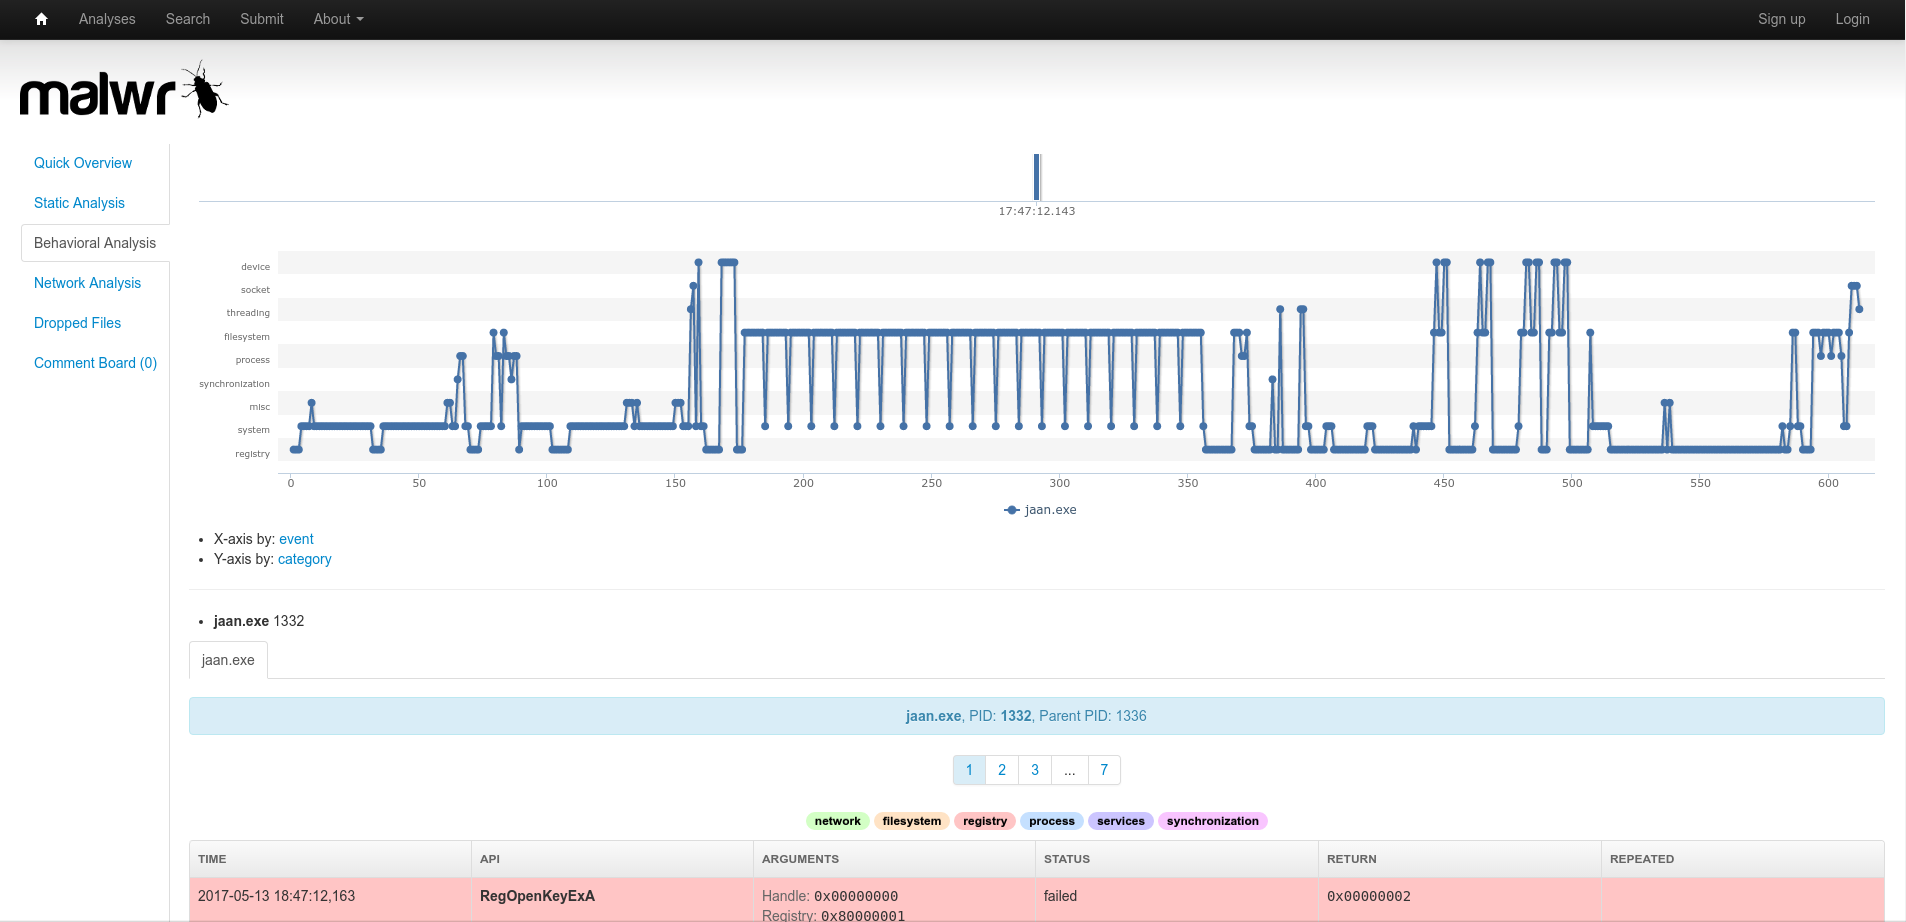
\includegraphics[width=\textwidth]{malwr_sample}
	\caption{Example of a behavioral report from Malwr}
	\label{fig:malwr_sample}
\end{figure}

For the purpose of detecting malware via \gls{ml}, the reports provided in Malwr supply various information that can be used to fulfill the current work. The whole website content is provided under \gls{cc} CC-BY-NC-SA 3.0\cite{cc-by-nc-sa} license, allowing the use of the data for this work's purpose, as long as credits are maintained.

%%%%%%%%%%%%%%%%%%%%%%%%%%%%%%%%%%%%%%%%%%%%%%%%%%%%%%%%%%%%%%%%%%%%%%%%%%%
%%%% Machine Learning
\subsection{Machine Learning}\label{subsec:ml}

Even before the modern concept of computer proposed by Alan Turing, mankind has always searched for ways to either automate or facilitate more complex tasks. With the technological advances that provide higher computation power, computer science fields like \gls{ai} have greatly improved in recent years. One of the \gls{ai} fields that has benefit from the technological advances is \gls{ml}. The current subsection will provide a more detailed description of \gls{ml} and its use for the current work.

\gls{ml} is a subset of \gls{ai} in which algorithms are applied to learn and make predictions on data, or more formally defined by Tom Mitchell\cite{mitchell:ml}:\\
\say{\emph{A computer program is said to learn from experience E with respect
		to some class of tasks T and performance measure P, if its performance at tasks in
		T, as measured by P, improves with experience E.}}

A noteworthy nuance about the given definition, and the \gls{ml} field in general, is that algorithms are not designed to deal with specific problems. Meaning that as long as a learning problem is well defined through $T$, $P$ and $E$, an algorithm based on these three features is able to learn, but not necessarily solve a problem.

After defining a learning problem, to obtain a useful outcome (i.e. model) one or more learning algorithms are applied. Learning algorithms fall within one of the following classes: supervised learning; unsupervised learning; semi-supervised learning or reinforcement learning. Each of the categories is defined on how the program learns the problem. A more detailed description, as seen in \cite{norvig:ai} is as follows:

\subsubsection{Supervised Learning.} In this category the program is given a corpus (i.e. experience) with input-output pairs and it must learn how to map a never seen input into the correct output. Within supervised learning, a learning problem can be further classified into a classification problem, if the output is a set of finite values (e.g. is it going to rain tomorrow?), or into a regression problem, if the output is continuous (e.g. how likely is it to rain tomorrow?).

\subsubsection{Unsupervised Learning.} In this category the program is given a corpus and it must learn patterns from the input, hence no correct or wrong output is expected, only how different input relates. The most common task in unsupervised learning is clustering, where input is grouped based on similar characteristics.

\subsubsection{Semi-supervised Learning.} This category is a combination of the previous ones and exists because sometimes the learning problem is based on a dataset that combines both labeled and unlabeled inputs or on a dataset that contains noisy data. The combination of supervised and unsupervised learning provides a better overall result in such scenarios.

\subsubsection{Reinforcement Learning.} In this category the program is given a problem through a set of states and a set of actions it can perform. At any given state the program performs an action which results in a reward or punishment. The cumulative reinforcement at each state teaches the program the best and worse actions for each state.\\

The proposed work will fit into the supervised learning category, with the purpose of creating a classifier to assert whether a given sample is malware or not. This problem can be seen as whether a pure classification problem, with a binary output, or as a regression problem, with the likelihood of a sample being malware.

When designing a learning system, multiple choices must be taken into consideration. A brief description of what should be taken into account is given as seen in\cite{mitchell:ml}.

The first choice is the \textit{training experience}, as it can have a significant impact on the success or failure of the learner. The feedback provided by the experience can be direct or indirect, affecting the end result of the system. Another important aspect is how the experience represents the distribution over which the performance is measured, meaning how well the experience represents the environment where the system is to be used.

The next choice is the \textit{target function}, representing what is to be learned. The function takes as input the set of features that represent the problem and (ideally) outputs a solution to the task.

With a well defined target function, what remains is \textit{choosing a representation for the target function}, where a learning model is applied to learn the given task. The choice is of great importance, given it will influence how well the system performs under evaluation.

Given the nature of the purposed work as a classification problem, many models can be applied as a representation for the target function. The following describe some models that should be taken into consideration during implementation.

\paragraph{Decision Tree Learning.}\cite{mitchell:ml} These methods are used to approximate discrete-valued target functions, where the learned function is represented as a decision tree. The decision tree is built based on how much information each attribute gives (i.e. information gain). These are best suited for problems where instances are represented by attribute-value pairs of discrete values and problems where data may contain errors. The shortcomings with decision tree methods include how deep to grow the decision tree, how to handle continuous attributes and handling attributes with different weights.

\paragraph{Artificial Neural Networks.}\cite{mitchell:ml} These methods can be used for real-valued, discrete-valued and vector-valued target functions. \gls{ann} are inspired in part by neurons in the biological world, hence being represented as directed graphs. \gls{ann}'s can be applied to the same type of problems as decision trees, but these can also handle instances represented by many attribute-value pairs. \gls{ann}'s have the downsides of being time consuming to train and to easily overfit the training data (i.e. training data is learned well, but fail to generalize to new data).

\paragraph{Bayesian Learning.}\cite{mitchell:ml} These methods use a probabilistic approach to inference. The reasoning is that the optimal decision can be related to some probabilistic distribution of the data. Bayesian learning proves to be effective for text classification tasks and also provides useful insight on other learning algorithms that do not deal with probabilities. The shortcomings can be related to the need of requiring initial knowledge, as well as computational cost to achieve the best hypothesis, which grows with the number of hypothesis.\\

Even though the field of \gls{ml} is broad, the main focus is always the ability to generalize a given task. For every learning task multiple models can be applied, which complicates the task of choosing a model. Being able to try different models how they compare to each other benefits the end result, which is to be taken into consideration for the current work.

%%%%%%%%%%%%%%%%%%%%%%%%%%%%%%%%%%%%%%%%%%%%%%%%%%%%%%%%%%%%%%%%%%%%%%%%%%
%%% Machine Learning in malware detection
\subsection{Machine Learning in Malware Detection}\label{subsec:ml_md}

The previous subsections gave a general understanding on how anti-virus software detects malware and how the \gls{ml} field can be applied to learn tasks without having to define specific algorithms. This section will describe research that aggregates both malware detection and machine learning. Authors make use of specific \gls{ml} classifiers like Naive Bayes (NB), \gls{lr} and \gls{svm} to design systems that learn to detect malware.

The main focus is to note the choices made by the authors relative to the datasets, classifiers and their evaluation, all of which are to be taken into consideration for the proposed work.

Before analyzing the work done with \gls{ml} in malware detection, it is worth noting how such work is to be conducted. Rossow et al\cite{rossow:practices} present some guidelines for designing malware experiments. Their work surveys 36 academic publications from 2006 to 2011 that rely on malware execution. The authors note frequent shortcomings in the surveyed publications regarding assumptions on the use of execution-driven datasets, absence of security precautions taken during experiments and insufficient description of the experimental setup. The provided guidelines are split into four groups: correct datasets, transparency, realism and safety.

Regarding correct datasets, the publication guidelines include whether goodware samples are to be present in datasets, how the dataset is balanced over malware families and if training and evaluation datasets should have different families. The authors note that at least nine distinct papers suffer from significant problems relating to the correctness criteria.

With regards to transparency, the given guidelines include the interpretation of false positives, false negatives and true positives, family names of employed malware samples and how they were named. In the surveyed papers, it is noted that the majority do not interpret the numeric results and a fifth do not name the malware families contained in the datasets.

Regarding realism, the paper introduces guidelines which include relevance and variety of malware families and real-world evaluations. The authors note that only a minority of papers include real-world evaluations and very few offer significant sample sizes, making it difficult to judge practical use of the methodology.

With regards to safety, the given guidelines focus on containment policies when analyzing malware samples. The authors note that most papers did not deploy or adequately describe containment.

As mentioned in subsection \ref{subsec:cuckoo}, the current work is to make use of the reports in Malwr, hence some the guidelines provided in the aforementioned research do not apply, specifically the safety guidelines. As for the other guidelines, it is important to take them into consideration when designing the proposed learning system.

On the same note of guidelines, Shabtai et al\cite{shabtai:survey} provide a survey directed at the application of machine learning classifiers to detect malware from static features. Their work concerns the design and evaluation of such systems. The process is divided into two phases: training and testing.

The training phase includes the creation of a vector to represent each file and posterior processing of such vectors to generate a classifier, while the testing phase measures the performance of the classifier by employing classical measures like \gls{tpr}, which measures the sensitivity (i.e. detection rate) of the classifier, and \gls{fpr}, which measures fall-out.

The authors outline that the work in designing learning systems include how the samples are to be represented (e.g. byte n-grams, portable executable features, strings), methods to select features (e.g. gain ratio, document frequency) and finally the classification algorithm (e.g. \gls{ann}, \gls{svm}).

It is noted by the authors that the use of multiple classifiers with different weights (ensembles) is beneficial to the classification task, as different classifiers work better on different features.

Some problems addressed that are of importance for the proposed work include the imbalance problem and chronological evaluation. Having a balanced dataset of malware and goodware does not accurately represent the real world. For chronological evaluation the question if whether the usage of old samples for training can aid or hinder the classification of new samples.

When it comes to malware detection from static features, Schultz et al\cite{schultz:data_mining} present a data-mining framework to detect new, unseen malicious executables. Their work uses a dataset of 4,266 programs, with 3,625 malicious binaries and 1,001 clean programs, labeled by a commercial anti-virus. The features include \gls{dll}'s used by the binary, list of \gls{dll} function calls, number of different function calls within each \gls{dll}, strings from the binary and byte sequences.

They apply three different models (RIPPER, Naive Bayes and Multi-Naive Bayes) to different features, achieving a detection rate between 52\% and 98\% and a false positive rate between 5\% and 9\%. It is worth noting how the application of different models to different features provide very distinct detection rates. Also worth noting is the size and imbalance of the dataset, where only 23\% of samples are benign in a total universe of 4,266 samples.

The authors describe the malware samples were obtained from various FTP sites and that 5\% were trojans, while the remaining 95\% consisted of viruses, with no remarks are made regarding the involved families. The majority of benign samples were gathered from a fresh installation of Windows 98, which may not represent the average benign sample.

Another application of \gls{ml} to malware detection from static features is done by Nissim et al\cite{nissim:al_pdf}. The authors apply active learning to the detection of malicious PDF files based on static features. They use a dataset of 6,774 PDF files, including 1629 malicious and 5,145 benign files, where the benign files were mark as such by Kaspersky anti-virus software.

Their framework works by filtering out all known benign and malicious PDF's and passing the remaining files to a \gls{svm} model, which linearly separates files based on an initial training set of malicious and benign files. The ones deemed informative are flagged for manual inspecting and used in future iterations of the \gls{svm} model training. The core idea in this work is to focus on detecting new and unseen instances of malware files with the help of human interaction.

The authors only apply an \gls{svm} model and justify its use due to previous work that provided good results in malware detection, the fact that it is hard for attackers to understand how the model separates files, that it is efficient when combined with active learning and the ability to handle large number of features.

They evaluate their framework by creating 10 subsets of 620 files, with the remaining 574 files used as initial training for the \gls{svm} model. For each subset the \gls{svm} is trained and choses the most informative files, these are manually inspected, labeled and added to the training set. By incrementally using a bigger training set with files manually labeled, the authors show a growing detection rate from 92\% in the first subset to nearly 97\% with the last subset. This is accompanied by a false positive rate from 0.6\% to under 0.2\%. These results show that their framework is capable of detecting new and unseen files without a very large training set, but with the help of manual inspection.

Their approach on creating subsets for evaluation and using more benign files in the sets can more closely relate to a real world scenario, as new malicious content is created every day, but it is still less then the amount of benign content.

The authors fail to describe why the chosen features work, this might be related to the use of an \gls{svm}, which makes it difficult interpret the parameters of the model.

With regards to malware detection from dynamic features, Rieck et al\cite{rieck:dynamic} propose a framework for automatic analysis of malware behavior using machine learning. Their approach applies both unsupervised (clustering) and supervised (classification) learning to identify novel malware classes and assign unknown to the discovered classes. Worth noting is that the mentioned work does not deal with goodware samples, focusing only on identifying different malware families.

Their framework starts by executing and monitoring the malware binaries in a sandbox environment, producing sequential reports that contain the operations and actions performed (system calls and their arguments). The reports are embedded in a high-dimensional vector space and \gls{ml} techniques for clustering and classification are applied.

To optimize the processing of reports, the authors propose a special representation of behavior, namely \gls{mist}. This representation encodes the monitored system call and its arguments using short numeric identifiers. Different levels of specificity can be obtained since the arguments are arranged in blocks. For variable-length arguments an index number is used, which can be mapped to the original content. Figure \ref{fig:mist} shows the schematic overview of \gls{mist} instructions.

\begin{figure}[h]
	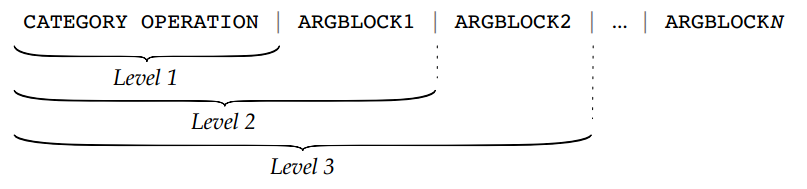
\includegraphics[width=\textwidth]{mist}
	\caption{\gls{mist} representation as seen in \cite{rieck:dynamic}}
	\label{fig:mist}
\end{figure}

An example of a MIST instruction could be as following:

\begin{center}\texttt{03 05 | 0100000001 | 00006ce5 | 000066fc}\end{center}

This instruction contains four levels. The first level contains the category and operation, while the remaining levels each contain an argument block. By variating the level, different granularities can be achieved.

The authors create a vector space for each report that represents the behavior of the sample. The vector is conceived by creating \textit{Q-grams}. These are the result of applying a sliding window of size $q$ to the MIST report and constructing a binary vector where every position is whether the report contains the sequence of size $q$ or not. The size of the vector varies with the number of possible instructions and the size $q$ of the window.

The authors implement their own clustering and classification algorithms for the task at hand. The evaluation data consists on two sets, a reference set of 3,133 malware reports with 24 different malware families, to be used to evaluate and calibrate the framework, and an application set of 33,698 unknown malware reports taken over a course of seven days.

On the reference set authors apply F-measure for evaluation, which uses precision and recall as parameters, the maximization of F-measure reflects high precison and recall. The results yield an F-measure over 0.936, which surpasses previous research for both clustering and classification.

On the application set authors apply their methodology and achieve 434 clusters (i.e. malware families). To the ten largest clusters authors take the most frequent anti-virus label for each cluster using Kaspersky anti-virus. They note that one anti-virus label is prevalent for each of the ten clusters, assuming that their framework successfully discovers and classifies unknown malware families.

By applying their framework to two different sets, where one was created from real-world samples, the authors show how their framework is applicable to a real-world scenario.

Miller et al\cite{miller:rev_int} provide a system which relates to \cite{nissim:al_pdf}, as it applies expert reviewers as a limited labeling resource. Their work uses both static and dynamic features to detect malware and uses manual label together with \gls{ml} to improve the overall result. The authors evaluate their design on an enormous dataset of 1.1 million binaries spanning 2.5 years, taken from submissions made at VirusTotal, a service similar to Malwr. Alongside the enormous dataset, the authors also make sure that training data predates evaluation data, contributing to an evaluation with high realism.

With regards to the design of the system, it consists of a detection and a training pipeline. The detection pipeline takes a binary, extracts the features and applies the current model to classify the binary as malicious or benign. The training pipeline takes binaries labeled by the manual reviewer, VirusTotal and from the current model, extracts the features and trains the new model.

The system uses multiple static and dynamic features from binaries, including: binary metadata, digital signing, static imports, dynamic imports, file operations, mutex operations, network operations, processes and Windows \gls{api} calls. The authors chose to use \gls{lr} as the classifier, basing their choice on the fact that it predicts a real-valued quantity, which enables the use of a threshold and therefore enables the creation of a tradeoff between true and false positive rates, by adjusting the threshold. \gls{lr} also assigns a weight to each feature, which allows to comprehend which features are more discriminating.

On evaluation, authors show that when ignoring temporal consistency, results inflate up to 20\% at a 0.5\% false positive rate. When considering temporal consistency, results range from 65\% to 75\% true positive rate with a false positive rate range from 0.1\% to 1\%.

Another remark made in this article is that vendors prefer false negatives over false positives (i.e. wrongly classifying malware as goodware over wrongly classifying goodware as malware). When looking at duplicated samples, 29.6\% of those samples increased in the number of detections as malware and only 0.25\% decreased the number of detections.

Perdisci et al\cite{perdisci:behavior} use an unsupervised learning approach to cluster malware using malicious network traces. Although their work does not directly relate to the proposed work, it also deals with the malware naming problem. To validate the obtained clusters, the cohesion and separation among clusters is measured in terms of the labels given by anti-virus vendors.

To derive the cohesion and separation, a graph for each cluster is constructed. Each node is a malware label given by some vendor and an edge connects two nodes if the labels appear together in any malware sample. Weights are assigned as $1 - \dfrac{m}{n}$, where $m$ is the number of times the different labels appear together and $n$ is the number of samples in the cluster. From the graphs the authors can then measure the cohesion and separation of clusters.

The authors use the aforementioned method to evaluate their results, but the approach can be useful to label and balance malware datasets that contain various anti-virus labels.\\

Overall the presented research provides useful insight for the current work. Decisions like the handling of the dataset, how and which features are to be extracted from samples, which and why \gls{ml} classifiers should be used and how and why the evaluation should be made.

%%%%%%%%%%%%%%%%%%%%%%%%
%%%%%%% SOLUTION %%%%%%%
%%%%%%%%%%%%%%%%%%%%%%%%
\section{Solution}\label{sec:solution}

With the knowledge given from previous sections, the current section will describe in detail the work be done as to achieve the objective of detecting malware samples by applying \gls{ml} classifiers.

As mentioned in section \ref{sec:introduction}, the approach to be taken to achieve the desired system is divided into three states: data collection, data labeling and classifier implementation. The following will describe each stage with more detail, together with work that as already been done.

\subsection{Data Collection}\label{subsec:data_collection}

The core objective of this stage is to obtain a corpus from which information about malware can be extracted. As mentioned in subsection \ref{subsec:cuckoo}, reports from Malwr are to be used, as they provide both static and dynamic information. The choice of using the already available reports instead of generating reports from collected samples is two-fold, it saves the overhead time of doing analysis and removes any bias regarding the sample choice, as real-world submissions are being used. The downside of using these reports is assuming the analysis was correctly done, which may not hold and can introduce noise to the extracted information.

The data provided by each report can be either static or dynamic, as mentioned in subsection \ref{subsec:cuckoo}. Malwr also provides additional information regarding static analysis, as it checks if the sample was submitted to VirusTotal, if so it lists the classification given by multiple anti-virus vendors. This information can then be used to assert if a sample is malicious or not.

Although Malwr enables the user to submit various type of objects, this work will only deal with \gls{pe} files (e.g. 32bit executables, \gls{dll}'s), as the Cuckoo implementation used by Malwr only provides static analysis for such files.

To check if the \gls{pe} provided a good amount of samples, an initial scrape of the list of analysis\footnote{Malwr Analysis List [https://malwr.com/analysis/]} was made using Scrapy\cite{tool:scrapy} and the present file types were analyzed. At the time of scrape there was a total of 642,698 submissions, where 388,702 (60.48\%) were \gls{pe} files, dated between April 16th, 2013 and October 10th, 2016. Figure \ref{fig:dist_submissions} and \ref{fig:dist_submissions_types} show the submissions by month, the percentage of duplicates per month and how the sample types are distributed, worth noting is that in August 2014 no samples were collected, possibly due to service downtime.

Knowing that \gls{pe} still account for a good part of all samples, a scrape of those reports was made. The reports were saved as HTML in the gzip format to save disk space. A total of 388,513 reports were obtained (different from the previous amount as some errors could have occurred during scraping) occupying a total of 26GB.

Having the reports locally, the next step is to parse the HTML format to extract the information to be used. Related work\cite{miller:rev_int,nissim:al_pdf,rieck:dynamic,schultz:data_mining,shabtai:survey} provide good examples of static and dynamic information to extract. So far only the static imports made by each executable were extracted (i.e. \gls{dll} functions), leaving much information to be extracted still. To speed parsing, Celery\cite{tool:celery} was used to distribute the work. Since it has proven to be useful in extracting static imports, it should also be applied for the remaining parsing.

\begin{figure}[!h]
	\subfloat[Total samples per month]{
		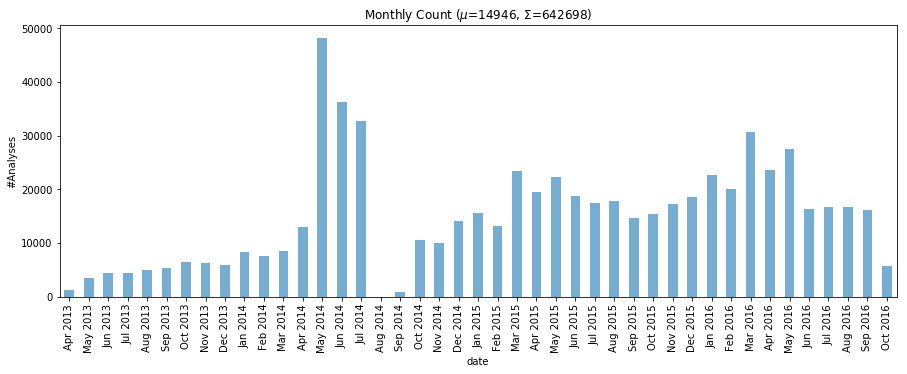
\includegraphics[width=\textwidth]{samples_count}
	}\\
	\subfloat[Percentage of duplicated (same MD5) samples per month]{
		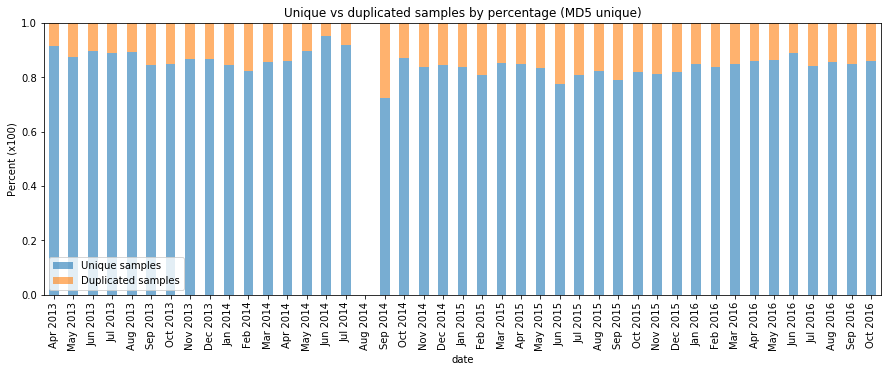
\includegraphics[width=\textwidth]{samples_dups}
	}
	\caption{Statistics for the scraped submissions. Count and percentage of duplicates}
	\label{fig:dist_submissions}
\end{figure}

\begin{figure}[!h]
	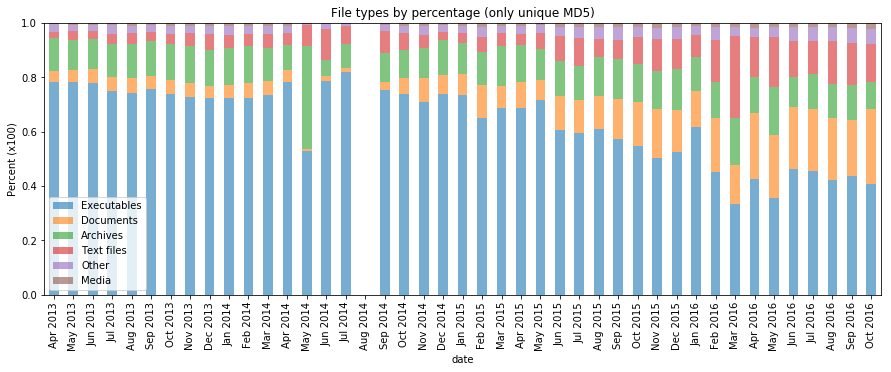
\includegraphics[width=\textwidth]{samples_types}
	\caption{Statistics for the scraped submissions. Distribution of file types}
	\label{fig:dist_submissions_types}
\end{figure}

\subsection{Data Labeling}\label{subsec:data_labeling}

While the previous section dealt with extracting information about an executable, the current section deals with labeling each executable as malicious or benign. This task is not trivial, as each sample is classified with different labels by different vendors. Not only that, but the number of anti-virus classifications varies among samples, as only vendors that have seen the sample classify it. Metrics have to be defined as to split the samples into malware or goodware.

To help labeling the dataset, this work proposes to filter samples by only keeping samples classified by a subset of vendors. The chosen subset is created by ordering the vendors by the number of classified samples (from the total number of samples) and choosing the top 20. This guarantees that every vendor has a classification for the sample at a reduced number of total samples.

To label a sample as benign, the current work defines that if a sample is considered as clean by all vendors, it is labeled as goodware. When dealing with duplicated samples, the most recent report is taken into account. Although this method may seen obvious in the first place, it can fail if at the time the report was made, vendors weren't able to detect the threat and labeled the sample benign. As authors in \cite{miller:rev_int} have shown, this problem occurred in almost 30\% of their duplicated samples.

To label a sample as malicious, the number of detections has to be taken into account. The imposed question is at which threshold should a sample be considered malware? On top of that, the type of malware should also be taken into consideration to provide a uniform (i.e balanced) dataset, as mentioned in \cite{rossow:practices}. A possible method to help balance the malware variety is to adopt some of the work in \cite{perdisci:behavior} regarding the naming problem: creating a graph where the nodes are all existing labels and edges connect each node based on how many times labels appear together in a sample.

Regarding data labeling some work was done to better understand the problem. For the top 20 anti-virus vendors, a filter was applied as to limit samples where all vendors classified as either goodware or malware, resulting in a total of 269,563 samples. A histogram of how many vendors classified a sample as malware was created, resulting in figure \ref{fig:dist_mal_class}. This shows how the threshold to label a sample as malware can be a difficult choice, since vendors often disagree on what is malware.

\begin{figure}[]
	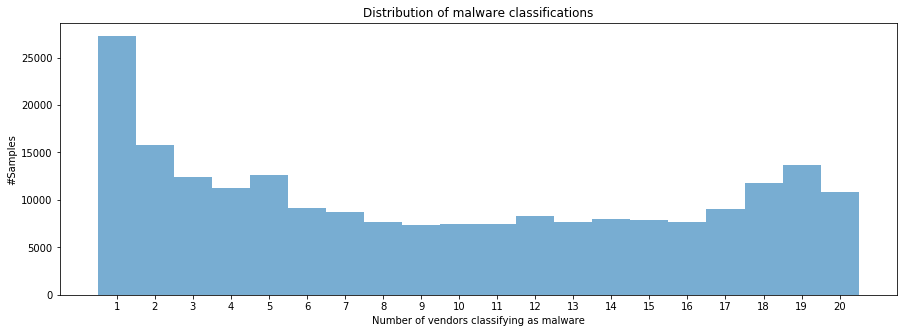
\includegraphics[width=\textwidth]{samples_top20_class}
	\caption{Distribution of how many vendors classify a sample as malware.}
	\label{fig:dist_mal_class}
\end{figure}

Further work was done to understand the naming variation. Again for the top 20 anti-virus vendors a filter was applied as to limit samples where all vendors classified as malware, resulting in a total of 10,868 (as can be seen in the last column of figure \ref{fig:dist_mal_class}). The unique number of names was counted, together with the percentage of repeating names. The results can be seen in table \ref{tab:statistics}, showing a varying number of unique names per vendor, with an average of 2,403 unique malware names per vendor. For the ten most repeating names, it can be seen that the variation is smaller and that on average the top ten most repeating names account for 28.7\% of the samples.


\subsection{Classifier Implementation}\label{subsec:class_implementation}

This final stage takes the work done in the previous stages to generate a model that is able to detect malware based on static and dynamic features. This stage is to take into consideration the guidelines given in \cite{rossow:practices,shabtai:survey} and the classifiers in \cite{miller:rev_int,nissim:al_pdf,rieck:dynamic,schultz:data_mining}. Ideally different classifiers should be tested, as some perform better over others for some set of features. The possibility of using multiple classifiers for different features can also be applied to improve the overall result.

\paragraph{Evaluation.} The final result is to be measured using the common evaluation metrics that others\cite{miller:rev_int,nissim:al_pdf,schultz:data_mining} have applied, specifically the \gls{tpr} and \gls{fpr}. The \gls{tpr} measures the detection rate of the resulting model, while the \gls{fpr} measures the fall-out.

The described metrics are to be applied in two different conditions: laboratory and real-world. For laboratory conditions, the dataset is to be randomly split, using one part for training and other for evaluation. For real-world conditions, the dataset is to be split by date, using older samples for training and more recent samples for evaluation. By forcing this temporal consistency, the current work will also try to validate the assumption in \cite{miller:rev_int}.

\subsection{Experimental Work}\label{subsec:exp_work}

As a motivation for the work still to be done, a small experiment was conducted to check how easily the creation of a classifier to detect malware is. A dataset was created using the static imports as features. As for the sample labeling, the classification as given by Microsoft's Windows Defender was used.

Using scikit-learn\cite{tool:sklearn} each sample was converted to a binary vector, where each position corresponded to the presence (or absence) of a static import. This feature representation lead to vectors with nearly 30,000 positions (i.e. there were almost 30,000 different static imports). A logistic regression classifier was trained with 75\% of the samples, using the remaining 25\% for evaluation. To check how the dataset balancing affected the classifier, as mentioned in \cite{rossow:practices}, three variants of the dataset were used.

The first dataset was the default and contained more goodware than malware (154,556 goodware, 76,495 malware), this yielded a detection rate 57.2\% with a \gls{fpr} of 28.4\%. The second dataset used the same amount of goodware and malware (76,495 samples each), resulting in a detection rate of 69.2\% and a \gls{fpr} of 23.7\%. The last dataset contained more malware than goodware (76,495 malware, 38,247 goodware) and gave a detection rate of 92\% with a \gls{fpr} of 22.4\%. Table \ref{tab:experimental} summarizes the results and notes the results from \cite{miller:rev_int} as a comparison.

\begin{table}[h!]
	\centering
	\def\arraystretch{1.5}
	\begin{tabular}{lcc}
		\toprule
		& Detection Rate        & False Positive Rate        \\
		\midrule
		First Dataset  & 0.572     & 0.284      \\ \hline
		Second Dataset & 0.692     & 0.237      \\ \hline
		Third Dataset  & 0.92      & 0.224      \\ \hline
		Miller et al   & [0.65, 0.75] & [0.001, 0.01] \\
		\bottomrule
	\end{tabular}
	\caption{Summary of experimental results compared to Miller et al\cite{miller:rev_int}}
	\label{tab:experimental}
\end{table}

This quick test gave some interesting results, although they do not compare to related work, it showed that with little to no work on the dataset and classifier a simple model was achieved. It also provided some experience with scikit-learn, which is to be used in the work to come.\\

The work that will result in the proposed system is to be developed between June 2017 and March 2018.

The planned schedule is to use the month of June to finish the data collection phase, together with the labeling phase during the months of June and July. The final phase of implementation is planned to take six months, from August to January, as many variables are present and more experiments should provide better results. Regarding the writing of the thesis document, the months of February and March are to be used. A more detailed planning can be seen in figure \ref{fig:schedule}.

\begin{figure}[h]
	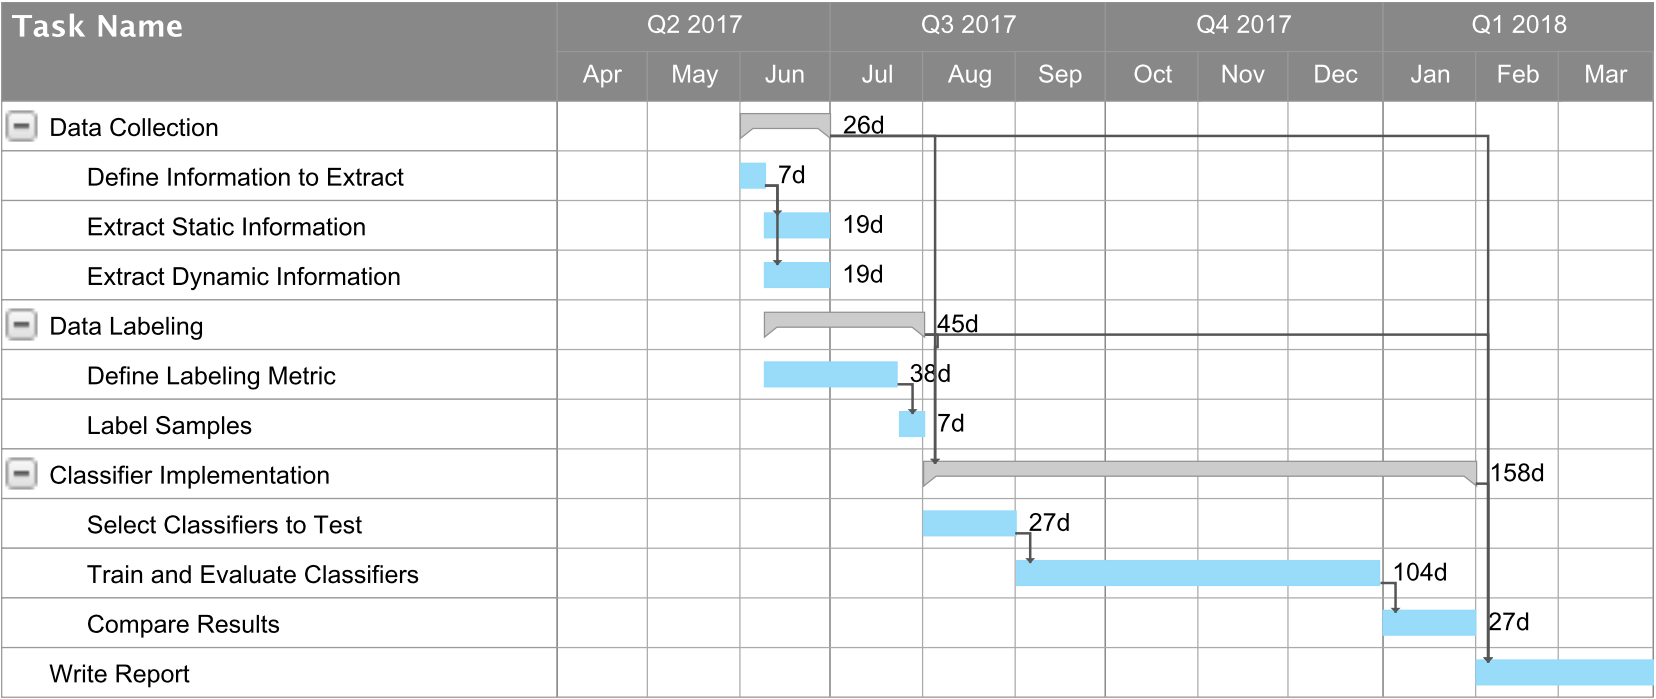
\includegraphics[width=\textwidth]{gantt}
	\caption{Planned Schedule}
	\label{fig:schedule}
\end{figure}


%%%%%%%%%%%%%%%%%%%%%%%%
%%%%%%%CONCLUSION%%%%%%%
%%%%%%%%%%%%%%%%%%%%%%%%
\section{Conclusion}\label{sec:conclusion}

With the growing amount of malware instances, being able to effectively detect malware as it appears is a must, otherwise cases like WannaCry malware\footnote{Wanna Cry Profile [https://www.fireeye.com/blog/threat-research/2017/05/wannacry-malware-profile.html]} will continue to have real and serious effects\footnote{Huffing Post Article [http://www.huffingtonpost.com/entry/britain-cyber-attack-national-health-service\_us\_5915e62ae4b00f308cf4fc86]}.

When new types of malware arise, anti-virus may be unable to detect them with the usual signature and heuristic methods. The application of \gls{ml} to the detection task as shown to be possible and effective\cite{kolter:learning,miller:rev_int,nissim:al_pdf,perdisci:behavior,rieck:dynamic,schultz:data_mining}. With that in mind, the current work will develop a \gls{ml} system capable of detecting malicious files, as well as test how different types of evaluations can impact the effectiveness of the solution.

The proposed solution, as described in section \ref{sec:solution}, is to be split in three steps: data collection, data labeling and classifier implementation. Some work as been done in each step as to get a feel on what to expect and the problems that might surge along the way.

The next step is to fully terminate each of the sequential stages, with special focus on classifier implementation as many variations can be tested, providing a better research and final result.

Hopefully the current work enlightened the reader on the problem, how the current technologies deal with it and how the proposed work could improve the detection task.

\begin{landscape}
	\begin{table}
		\centering
		\def\arraystretch{1.1}
		\subfloat{
			\begin{tabular}{rcccccccccc}
				\toprule
				{} &  thehacker &  bitdefender &  cat-quickheal &  fortinet &   virobot &    ikarus &     gdata &    f-prot &  k7antivirus &    clamav \\
				\midrule
				Unique names   &   3090 &     3223 &       2286 &  2144 &  3617 &  1139 &  3227 &  2515 &     1869 &  3195 \\
				\midrule
				1st most used  &      0.068 &        0.066 &          0.063 &     0.057 &     0.063 &     0.075 &     0.066 &     0.052 &        0.042 &     0.026 \\
				2nd most used  &      0.047 &        0.047 &          0.052 &     0.050 &     0.028 &     0.040 &     0.047 &     0.035 &        0.035 &     0.022 \\
				3rd most used  &      0.039 &        0.029 &          0.040 &     0.032 &     0.027 &     0.028 &     0.029 &     0.032 &        0.030 &     0.022 \\
				4th most used  &      0.030 &        0.025 &          0.030 &     0.027 &     0.025 &     0.027 &     0.025 &     0.030 &        0.029 &     0.017 \\
				5th most used  &      0.025 &        0.020 &          0.028 &     0.027 &     0.022 &     0.023 &     0.020 &     0.029 &        0.023 &     0.017 \\
				6th most used  &      0.021 &        0.019 &          0.024 &     0.025 &     0.015 &     0.021 &     0.019 &     0.028 &        0.023 &     0.017 \\
				7th most used  &      0.019 &        0.017 &          0.023 &     0.019 &     0.013 &     0.017 &     0.017 &     0.026 &        0.023 &     0.017 \\
				8th most used  &      0.018 &        0.017 &          0.021 &     0.018 &     0.013 &     0.016 &     0.017 &     0.019 &        0.021 &     0.015 \\
				9th most used  &      0.015 &        0.017 &          0.019 &     0.017 &     0.012 &     0.015 &     0.017 &     0.017 &        0.020 &     0.014 \\
				10th most used &      0.015 &        0.014 &          0.014 &     0.015 &     0.012 &     0.015 &     0.014 &     0.015 &        0.018 &     0.013 \\
				\midrule
				Total          &      0.297 &        0.272 &          0.315 &     0.287 &     0.231 &     0.277 &     0.272 &     0.283 &        0.263 &     0.179 \\
				\bottomrule
			\end{tabular}
		}\\
		\subfloat{
			\begin{tabular}{rcccccccccc}
				\toprule
				{} &    mcafee &  microsoft &  nprotect &    comodo &     avast &       avg &     vba32 &  kaspersky &  mcafee-gw-edition &  symantec \\
				\midrule
				Unique names   &  2560 &   1644 &  4332 &  1959 &  1570 &  2644 &  1366 &   2572 &           2436 &   667 \\
				\midrule
				1st most used  &     0.069 &      0.064 &     0.060 &     0.068 &     0.068 &     0.044 &     0.069 &      0.064 &              0.051 &     0.071 \\
				2nd most used  &     0.037 &      0.040 &     0.030 &     0.061 &     0.062 &     0.032 &     0.030 &      0.052 &              0.036 &     0.060 \\
				3rd most used  &     0.030 &      0.030 &     0.025 &     0.050 &     0.058 &     0.031 &     0.025 &      0.046 &              0.024 &     0.060 \\
				4th most used  &     0.030 &      0.028 &     0.020 &     0.036 &     0.043 &     0.025 &     0.025 &      0.041 &              0.024 &     0.053 \\
				5th most used  &     0.028 &      0.027 &     0.018 &     0.031 &     0.042 &     0.023 &     0.023 &      0.030 &              0.019 &     0.033 \\
				6th most used  &     0.028 &      0.025 &     0.016 &     0.028 &     0.030 &     0.017 &     0.022 &      0.028 &              0.018 &     0.032 \\
				7th most used  &     0.024 &      0.025 &     0.016 &     0.027 &     0.024 &     0.017 &     0.017 &      0.025 &              0.017 &     0.032 \\
				8th most used  &     0.019 &      0.025 &     0.014 &     0.021 &     0.019 &     0.017 &     0.016 &      0.021 &              0.016 &     0.030 \\
				9th most used  &     0.017 &      0.020 &     0.014 &     0.019 &     0.019 &     0.015 &     0.016 &      0.020 &              0.013 &     0.028 \\
				10th most used &     0.017 &      0.019 &     0.013 &     0.015 &     0.017 &     0.015 &     0.013 &      0.019 &              0.012 &     0.026 \\
				\midrule
				Total          &     0.300 &      0.304 &     0.228 &     0.356 &     0.383 &     0.237 &     0.258 &      0.345 &              0.230 &     0.425 \\
				\bottomrule
			\end{tabular}
		}
	\caption{Malware name statistics for samples where all top 20 vendors classify as malware (10,868 samples). Tables show the unique different names together with repeating names percentage.}
	\label{tab:statistics}	
	\end{table}
\end{landscape}


%%%%%%%%%%%%%%%%%%%%%%%%
%%%%%%%REFERENCES%%%%%%%
%%%%%%%%%%%%%%%%%%%%%%%%
\clearpage
\nocite{*}
\bibliography{reportbib}{}
\bibliographystyle{plain}

\end{document}